\documentclass[12pt]{exam}
\usepackage[margin=0.5in]{geometry}
\usepackage{amsmath,amssymb}
\usepackage{multicol}
\usepackage{tikz}
\usetikzlibrary{arrows,automata,positioning}
\usepackage{soul}
\usepackage{tcolorbox,minted} % For python code syntax highlighting

\newcommand{\blank}[1]{\underline{\hspace*{#1}}}
\newcommand{\ds}{\displaystyle}
\newcommand{\on}{\operatorname}
\newcommand{\mymod}{~\mathrm{mod}~}
\newcommand{\N}{\mathbb{N}}


\begin{document}
\pagestyle{empty}
\graphicspath{{/home/brian/Dropbox/HSC/Spring16/Math111/}}

\subsubsection*{COMS 461 - Midterm 3 Review}

%\begin{itemize}
%\item Big-O notation - true/false comparisons; identify running time of an algorithm using Big-O.
%\item Class P - 
%\item Class NP - prove that a language is in class NP by describing a verifier, maybe follow a nondeterministic algorithm to see if it is polynomial time.
%\item Polynomial time reductions - maybe prove that a polynomial time reduction exists, or prove a more abstract result assuming that a reduction exists. 
%\item NP-complete \& NP-hard 
%\item SAT problem \& Cook-Levin theorem 
%\end{itemize}

\begin{questions}

\question[8] Is the following Boolean formula satisfiable? Explain.
$$(x \vee y) \wedge (x \vee \bar{y}) \wedge (\bar{x} \vee y) \wedge (\bar{x} \vee \bar{y})$$
\begin{solution}
No, it is not satisfiable. No matter what Boolean values you pick for $x$ and $y$, one of the clauses will have both of its literals false.  
\end{solution}
\vfill


\question[16] A Boolean formula in conjugate normal form can be converted to a multivariable polynomial with integer coefficients so that the Boolean formula is satisfiable if and only if the polynomial has an integer root.  Here is how:
\begin{itemize}
\item Convert any non-negated variable $x$ to $(1-x)^2$.
\item Convert a negated variable $\bar{x}$ to $x^2$. 
\item Convert each $\vee$ into multiplication ($*$). 
\item Convert each $\wedge$ into addition $(+)$. 
\end{itemize}
\begin{parts}
\part Use these steps to convert the Boolean formula
$$(x \vee y) \wedge (x \vee \bar{y}) \wedge (\bar{x} \vee y) \wedge (\bar{x} \vee \bar{y})$$
into an integer polynomial.  You do not need to simplify the polynomial. 
\begin{solution}
$$\left(1-x\right)^{2}\left(1-y\right)^{2}+\left(1-x\right)^{2}y^{2}+x^{2}\left(1-y\right)^{2}+x^{2}y^{2}$$
\end{solution}
\vfill

%\part Let $\phi$ be a Boolean formula in CNF. If $\phi \in \text{SAT}$, then show that the corresponding polynomial $p_\phi$ has an integer root.  
%\begin{solution}
%By using 1 for true and 0 for false, we can plug into the formulas in 
%\end{solution}
%\vfill

\part Let $\text{INTEGER-ROOT} = \{\langle p \rangle \, : \, p \text{ is a multivariate integer polynomial with an integer root} \}.$ \\
Given that we can convert Boolean formulas to integer polynomials as described above, which of the following is true?
\begin{choices}
\CorrectChoice $\text{SAT} \le_p \text{INTEGER-ROOT}$.
\choice $\text{INTEGER-ROOT} \le_p \text{SAT}$.
\choice Both. $\text{INTEGER-ROOT}$ and $\text{SAT}$ are polynomial-time equivalent.
\choice Neither. $\text{SAT} \nleq_p \text{INTEGER-ROOT}$ and $\text{INTEGER-ROOT} \nleq_p \text{SAT}$.
\end{choices}
\bigskip

\part It turns out that INTEGER-ROOT is Turing recognizable, but not decidable. Which of the following complexity classes does INTEGER-ROOT belong to?  If it is in more than one, choose the smallest one.
\begin{choices}
\choice P
\choice NP
\choice NP-complete
\choice EXP
\CorrectChoice NP-hard
\end{choices}
\end{parts}
\bigskip
\newpage


\question[16] For each of the following, determine if the statement is true or false.  Briefly explain your answers.
\begin{multicols}{2}
\begin{parts}
\part $\log n \in O(n)$. \\ \vspace*{1.0in}
\part $n^2 \log n \in O(n^2)$. \\ \vspace*{1.0in}
\part $n^3 + \log n \in O(n^3)$. \\ \vspace*{1.0in}
\part $n^n \in O(2^{(n^2)})$.  \\ \vspace*{1.0in}
\end{parts}
\end{multicols}
\begin{solution}
(a) True, (b) False, (c) True, (d) True, since $2^{(n^2)} = (2^n)^n > n^n$.
\end{solution}

\question[12] Let $f: \{1, \ldots, N \} \rightarrow \{1, \ldots, N\}$ be an invertible function such that when these integers are represented in binary, $f$ can be computed in polynomial time, but $f^{-1}$ cannot be computed in polynomial time.  Let 
$$L = \{ (x,y) \, : \, f^{-1}(x) \le y \}.$$
\begin{parts}
\part Explain why $L \in \text{NP}$. 
\begin{solution}
A solution for $L$ would be $s = f^{-1}(x)$.  Then you would just have to check that (i) $f(s) = x$ and (ii) $s \le y$, both of which can be done in polynomial time. So $L$ has a polynomial time verifier. 
\end{solution}
\vfill

%\part Prove that $L \notin \text{P}$. 
%\begin{solution}
%If $L \in \text{P}$, then you could use a divide and conquer algorithm to figure out $f^{-1}(x)$ in polynomial time by trying different values of $y$ to find which are bigger than $f^{-1}(x)$. The would contradict the assumption that $f^{-1}$ cannot be computed in polynomial time. 
%\end{solution} 
%\vfill

\part The assumptions above imply that $L \notin P$. Why is this not a proof that $\text{P} \neq \text{NP}$? 
\begin{choices}
\choice Because one example is not enough to prove that $\text{P} \neq \text{NP}$.
\choice Because $L$ might not be NP-complete.
\CorrectChoice Because there might not be a function $f$ with the properties described above.
\choice Because $L$ is not decidable.  
\end{choices}
\vfill
\end{parts}

\question[8] What does the Cook-Levin theorem say about SAT?  
\begin{solution}
It says that SAT is NP-complete.
\end{solution}
\vfill

\newpage
\question[12] Let $\text{NO-REPEATS} = \{\langle A \rangle \, : \, A \text{ is an integer array with no repeat entries}\}.$
\begin{parts}
\part The following algorithm decides if an array $A$ of integers is in NO-REPEATS.  What is the Big-O run time of this algorithm? Use $n$ to denote the length of the input (encoded in binary).  You can assume that any two integers with binary lengths less than $n$ can be compared in $O(n)$ time. 

\begin{tcolorbox}
\begin{minted}{python}
let k = length(A)
# Loop through pairs of entries in A to see if any are the same:
for i from 1 to k-1: 
  for j from i+1 to k:
    if A[i] == A[j]:
      return False
# If you don't find any entries of A that are the same:
return True
\end{minted}
\end{tcolorbox}
\begin{solution}
$$O(n^3)$$
\end{solution}
\vfill


\part Which of the following complexity classes does NO-REPEATS belong to?  If it is in more than one, choose the smallest one.
\begin{choices}
\CorrectChoice P
\choice NP
\choice NP-complete
\choice EXP
\choice NP-hard
\end{choices}
\end{parts}
\bigskip

%\question Let $\text{IN-ORDER} = \{\langle x_1, \ldots, x_k \rangle \, : \, \text{ each $x_i$ is an integer and $x_{i} \le x_{i+1}$ for all $i$}\}.$
%\begin{parts}
%\part Write an algorithm in psuedocode to decide if a list of numbers $\langle x_1, \ldots, x_k \rangle$ is in the language IN-ORDER. 
%\vfill
%
%\part Assuming that we can compare integers in $O(n)$ time (where $n$ is the length of the input), what is the running time for your algorithm in Big-O notation? 
%\vfill
%
%\part Which of the following complexity classes does IN-ORDER belong to?  If it is in more than one, choose the smallest one.
%\begin{choices}
%\choice P
%\choice NP
%\choice NP-complete
%\choice EXP
%\choice NP-hard
%\end{choices}
%\end{parts}
%\bigskip


\question[8] A graph is 3-colorable if you can assign one of three colors to each of the vertices in such a way that no edge connects two vertices with the same color.  Let 
$$\text{3-COLORABLE} = \{ \langle G \rangle \, : \, G \text{ is a 3-colorable graph}\}.$$ 
Is it possible to create a nondeterministic polynomial-time algorithm to decide 3-COLORABLE? You do not have to find an algorithm, just explain why such an algorithm does or does not exist.
\begin{solution}
It is easy to see that 3-COLORABLE is in class NP since a proposed coloring can be checked in polynomial time by looping through the edges and checking the colors of its vertices.  Therefore there must be a nondeterministic polynomial time algorithm to decide 3-coloring. 
\end{solution}
\vfill
\vfill
\vfill

\newpage
\question[20] A graph $G$ has a Hamiltonian cycle if there is a path that (i) starts and ends at the same vertex, and (ii) visits every other vertex exactly one. For example the graph on the left below has a Hamilton cycle ($1 \rightarrow 2 \rightarrow 3 \rightarrow 4 \rightarrow 1$), but the graph on the right does not. 
\begin{center}
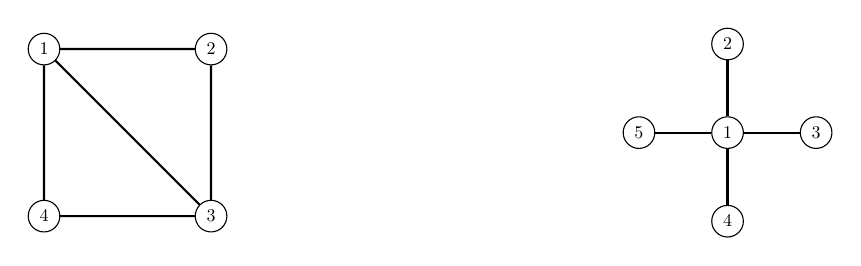
\begin{tikzpicture}[scale=1.5]
\path  (135:1) node[draw,shape=circle,scale=0.65] (B1) {1};
\path (45:1)   node[draw,shape=circle,scale=0.65] (B2) {2};
\path (-45:1)  node[draw,shape=circle,scale=0.65] (B3) {3};
\path (-135:1) node[draw,shape=circle,scale=0.65] (B4) {4};

\draw[thick] (B1) to (B2);
\draw[thick] (B2) to (B3);
\draw[thick] (B3) to (B4);
\draw[thick] (B4) to (B1);
\draw[thick] (B1) to (B3);

\begin{scope}[xshift=2in]
\path  (45:0)  node[draw,shape=circle,scale=0.65] (C1) {1};
\path  (90:0.75)  node[draw,shape=circle,scale=0.65] (C2) {2};
\path (0:0.75)    node[draw,shape=circle,scale=0.65] (C3) {3};
\path (-90:0.75)  node[draw,shape=circle,scale=0.65] (C4) {4};
\path (-180:0.75) node[draw,shape=circle,scale=0.65] (C5) {5};

\draw[thick] (C1) to (C2);
\draw[thick] (C1) to (C3);
\draw[thick] (C1) to (C4);
\draw[thick] (C1) to (C5);

\end{scope}
\end{tikzpicture}
\end{center}
\begin{parts}
\part Find a Hamiltonian cycle for the graph below (there is more than one right answer). \\
\begin{center}
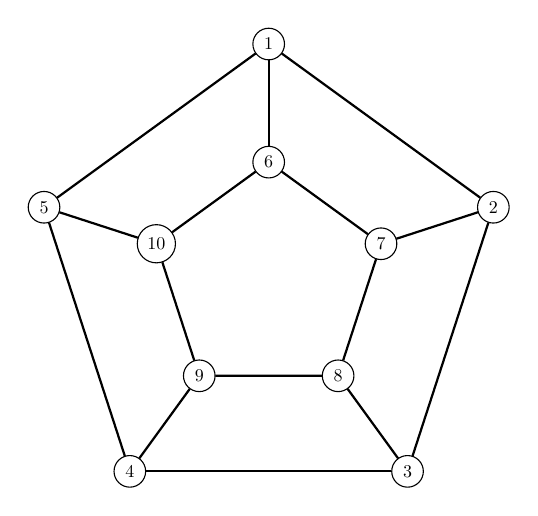
\begin{tikzpicture}[scale=1.5]
\path (90:2)   node[draw,shape=circle,scale=0.65] (B1) {1};
\path (18:2)   node[draw,shape=circle,scale=0.65] (B2) {2};
\path (-54:2)  node[draw,shape=circle,scale=0.65] (B3) {3};
\path (-126:2) node[draw,shape=circle,scale=0.65] (B4) {4};
\path (-198:2) node[draw,shape=circle,scale=0.65] (B5) {5};
\path (90:1)   node[draw,shape=circle,scale=0.65] (C1) {6};
\path (18:1)   node[draw,shape=circle,scale=0.65] (C2) {7};
\path (-54:1)  node[draw,shape=circle,scale=0.65] (C3) {8};
\path (-126:1) node[draw,shape=circle,scale=0.65] (C4) {9};
\path (-198:1) node[draw,shape=circle,scale=0.65] (C5) {10};

\draw[thick] (B1) to (B2);
\draw[thick] (B2) to (B3);
\draw[thick] (B3) to (B4);
\draw[thick] (B4) to (B5);
\draw[thick] (B5) to (B1);

\draw[thick] (B1) to (C1);
\draw[thick] (B2) to (C2);
\draw[thick] (B3) to (C3);
\draw[thick] (B4) to (C4);
\draw[thick] (B5) to (C5);

\draw[thick] (C1) to (C2);
\draw[thick] (C2) to (C3);
\draw[thick] (C3) to (C4);
\draw[thick] (C4) to (C5);
\draw[thick] (C5) to (C1);
\end{tikzpicture}
\end{center}
\bigskip

\part Let $\text{HAMILTON-CYCLE} = \{ \langle G \rangle \, : \, G \text{ is a graph with a Hamilton cycle} \}.$ Prove that the language $\text{HAMILTON-CYCLE} \in \text{NP}$ by describing a polynomial-time verifier. 
\begin{solution}
The verifier would input both a graph $G$, and an ordered list of vertices in a Hamiltonian cycle.  It would then traverse the list and make sure that (i) every vertex gets visited exactly once, (ii) the path ends where it started, and (iii) every step corresponds to an edge in the graph.  This would require only one loop through the solution string, marking each vertex in the graph as it gets visited, and then a final loop to check that each vertex is marked exactly once.  So this would run in polynomial time. 
\end{solution}
\vfill

\part The language HAMILTON-CYCLE is actually NP-complete.  What does this mean about its relationship with the language SAT?  
\begin{choices}
\choice $\text{SAT} \le_p \text{HAMILTON-CYCLE}$, but $\text{HAMILTON-CYCLE} \nleq_p \text{SAT}$.
\choice $\text{HAMILTON-CYCLE} \le_p \text{SAT}$, but $\text{SAT} \nleq_p \text{HAMILTON-CYCLE}$.
\CorrectChoice $\text{SAT} \leq_p \text{HAMILTON-CYCLE}$ and $\text{HAMILTON-CYCLE} \leq_p \text{SAT}$.
\choice $\text{HAMILTON-CYCLE} \nleq_p \text{SAT}$ and $\text{SAT} \nleq_p \text{HAMILTON-CYCLE}$.
\end{choices}
\end{parts}
\bigskip
\end{questions}

\end{document}
